\documentclass[12pt,letterpaper]{article}

\usepackage[margin=0.85in]{geometry}
\usepackage[T1]{fontenc}
\usepackage{lmodern}
\usepackage[scaled=0.95]{helvet}
\renewcommand{\familydefault}{\sfdefault}
\usepackage{amsmath}
\usepackage{array}
\usepackage{tabularx}
\usepackage[table]{xcolor}
\usepackage{tikz}
\usetikzlibrary{arrows.meta}
\usepackage[most]{tcolorbox}
\usepackage{titlesec}
\usepackage{fancyhdr}
\usepackage{needspace}

% ---------- Colors ----------
\definecolor{monster}{HTML}{1F6FB5}   % Cookie Monster blue
\definecolor{cookiedark}{HTML}{7A4A22}
\definecolor{elmo}{HTML}{D32F2F}
\definecolor{oscar}{HTML}{4C8C2B}
\definecolor{count}{HTML}{6B3FA0}     % The Count purple
\definecolor{cookie}{HTML}{C68B4E}
\definecolor{chip}{HTML}{3B2314}
\definecolor{softyellow}{HTML}{FFF6DD}
\definecolor{softblue}{HTML}{E8F1FA}
\definecolor{softpurple}{HTML}{F1EBF8}
\definecolor{softgreen}{HTML}{EDF5E8}
\definecolor{gold}{HTML}{C68B4E}
\definecolor{snuffy}{HTML}{8D5B3E}    % Snuffy brown
\definecolor{bigbird}{HTML}{B8860B}   % Big Bird yellow, darkened for print
\definecolor{softbrown}{HTML}{F6EEE8}

% ---------- Headings ----------
\titleformat{\section}{\Large\bfseries\color{cookiedark}}{}{0pt}{}
\titlespacing*{\section}{0pt}{14pt}{6pt}
\setcounter{secnumdepth}{0}

\pagestyle{fancy}
\fancyhf{}
\renewcommand{\headrulewidth}{0pt}
\fancyfoot[C]{\small\color{gray}The Count's Square Cookies \textperiodcentered\ page \thepage}

\setlength{\parindent}{0pt}
\setlength{\parskip}{6pt}

% ---------- Helpers ----------
% A cookie with chocolate chips
\newcommand{\cookie}[1][1]{%
  \begin{tikzpicture}[scale=#1, baseline=-0.6ex]
    \fill[cookie] (0,0) circle (0.5);
    \draw[cookiedark, line width=0.8pt] (0,0) circle (0.5);
    \foreach \x/\y in {-0.2/0.2, 0.15/0.25, 0.25/-0.1, -0.1/-0.25, -0.28/-0.05, 0.05/0.0}
      \fill[chip] (\x,\y) circle (0.06);
  \end{tikzpicture}}

% A square tray of #1 x #1 cookies
\newcommand{\tray}[1]{%
  \begin{tikzpicture}[baseline=(current bounding box.south)]
    \draw[cookiedark, line width=1pt, fill=softyellow, rounded corners=2pt]
      (-0.3,-0.3) rectangle (#1*0.5-0.2, #1*0.5-0.2);
    \foreach \r in {1,...,#1}
      \foreach \c in {1,...,#1}
        \node[inner sep=0pt] at (\c*0.5-0.5, \r*0.5-0.5) {\cookie[0.42]};
  \end{tikzpicture}}

\newcommand{\blank}[1][3cm]{\underline{\hspace{#1}}}

\newcounter{question}
\newcommand{\question}{%
  \refstepcounter{question}\par\needspace{3\baselineskip}%
  \textbf{\color{monster}Question \arabic{question}.}~}

\newtcolorbox{bigidea}[1][]{enhanced, colback=softyellow, colframe=gold,
  boxrule=1pt, arc=3mm, left=8pt, right=8pt, top=6pt, bottom=6pt, #1}
\newtcolorbox{tryit}{enhanced, colback=softblue, colframe=monster,
  boxrule=0.8pt, arc=3mm, left=8pt, right=8pt}
\newtcolorbox{oscarbox}{enhanced, colback=softgreen, colframe=oscar,
  boxrule=1pt, arc=3mm, left=8pt, right=8pt, top=6pt, bottom=6pt}
\newtcolorbox{snuffybox}{enhanced, colback=softbrown, colframe=snuffy,
  boxrule=1pt, arc=3mm, left=8pt, right=8pt, top=6pt, bottom=6pt}
\newtcolorbox{mathclub}[1]{enhanced, colback=softpurple, colframe=count,
  boxrule=0.8pt, arc=3mm, left=8pt, right=8pt, top=4pt, bottom=4pt,
  title={\textbf{#1}}, colbacktitle=count, coltitle=white}

\renewcommand{\arraystretch}{1.6}

\begin{document}

% ================= Title =================
\begin{center}
  {\cookie[0.9]\hspace{0.6em}\cookie[0.9]\hspace{0.6em}\cookie[0.9]}\\[6pt]
  {\Huge\bfseries\color{cookiedark} The Count's Square Cookies}\\[4pt]
  {\Large Where $j = \sqrt{-1}$ Comes From}\\[6pt]
  {\small\color{gray} November 4, 2026 \textperiodcentered\ Nathaniel}
\end{center}

\vspace{2pt}
Name: \blank[6cm] \hfill Date: \blank[4cm]

% ================= The story =================
\section{The story}

\textbf{\color{count}The Count} loves squares. Every night he puts cookies on trays in perfect
squares, with the same number of cookies in every row and column. \emph{``Ah ah ah!''}

\textbf{\color{monster}Cookie Monster} just wants to eat them. \textbf{\color{oscar}Oscar the
Grouch} just wants to cause trouble. And tonight, Oscar asks The Count for a tray so strange
that nobody has ever seen one. To make it, we will need a brand new number called $j$, and
help from \textbf{\color{bigbird}Big Bird}'s best friend, \textbf{\color{snuffy}Mr.\ Snuffleupagus}.
Snuffy for short!

% ================= Square trays =================
\section{Square trays}

\begin{center}
\begin{tabular}{c@{\hspace{2.2em}}c@{\hspace{2.2em}}c}
\tray{1} & \tray{2} & \tray{3} \\[2pt]
1 row of 1 & 2 rows of 2 & 3 rows of 3 \\
$1 \times 1 = 1$ cookie & $2 \times 2 = 4$ cookies & $3 \times 3 = 9$ cookies \\
\end{tabular}
\end{center}

\question Fill in The Count's tray table. You can draw the trays or use counters.

\begin{center}
\renewcommand{\arraystretch}{1.3}
\rowcolors{2}{white}{softyellow}
\begin{tabular}{|>{\centering\arraybackslash}p{4.2cm}|>{\centering\arraybackslash}p{3.2cm}|>{\centering\arraybackslash}p{3.6cm}|}
\hline
\rowcolor{cookiedark}
\textbf{\color{white}Cookies on each side} & \textbf{\color{white}Times itself} & \textbf{\color{white}Cookies on tray} \\
\hline
1 & $1 \times 1$ & 1 \\ \hline
2 & $2 \times 2$ & 4 \\ \hline
3 & $3 \times 3$ & 9 \\ \hline
4 & $4 \times 4$ &   \\ \hline
5 & $5 \times 5$ &   \\ \hline
\end{tabular}
\end{center}

\begin{bigidea}
A number times \textbf{itself} is called a \textbf{square}, because it makes a square tray.
We write $3 \times 3$ as $3^2$ and say \textbf{``three squared.''}
\end{bigidea}

% ================= Square roots =================
\newpage
\section{Going backwards: the square root}

Cookie Monster finds a tray of cookies. He wants to know: \emph{``How many cookies on each side?
Me need to know where to start!''}

\begin{bigidea}
The \textbf{square root} goes backwards. It starts with the cookies on the tray and finds the
side. We write it with a check-mark sign:
\[
  \sqrt{9} \quad\text{means}\quad \text{``what number times itself makes 9?''}
\]
$3 \times 3 = 9$, so $\sqrt{9} = 3$. Say it: \textbf{``the square root of nine is three.''}
\end{bigidea}

\question Use the tray table to go backwards.

\begin{center}
\renewcommand{\arraystretch}{2}
\begin{tabular}{l@{\hspace{3em}}l@{\hspace{3em}}l}
$\sqrt{4} = $ \blank[1.5cm] & $\sqrt{16} = $ \blank[1.5cm] & $\sqrt{25} = $ \blank[1.5cm] \\
$\sqrt{1} = $ \blank[1.5cm] & $\sqrt{100} = $ \blank[1.5cm] & \\
\end{tabular}
\end{center}

\begin{tryit}
\textbf{Try it!} Get 12 counters. Can you make a square tray with all 12, with no counters left
over? Now try 16.
\end{tryit}

\question Which one makes a square tray: 12 or 16? \blank[2cm]

% ================= Oscar's surprise =================
\section{Oscar's surprise}

\begin{oscarbox}
\textbf{\color{oscar}Oscar the Grouch:} \emph{``Scram! I know ANOTHER number that times itself
makes 9!''}

Remember Oscar's opposite trick: an opposite of an opposite takes you back.
So a negative times a negative is \textbf{positive}:
\[
  (-3) \times (-3) = 9 .
\]
\end{oscarbox}

\question $(-4) \times (-4) = $ \blank[2cm]

\vspace{4pt}
\question Find \textbf{two} numbers that make 25 when you multiply them by themselves.\\[4pt]
\blank[1.5cm] and \blank[1.5cm]

\begin{bigidea}
So 9 has \textbf{two} square roots: $3$ and $-3$. To keep things simple, everyone agreed that
the sign $\sqrt{\phantom{9}}$ means the \textbf{plus} one: $\sqrt{9} = +3$. Remember this rule.
It comes back at the end!
\end{bigidea}

% ================= The impossible tray =================
\newpage
\section{Oscar's impossible tray}

\emph{``Count! Make me a square tray of \textbf{minus one} cookie!''} That means we need
$\sqrt{-1}$: \textbf{a number that times itself makes $\boldsymbol{-1}$}.

The Count tries every number he knows. \emph{``Ah ah ah! Let me count them!''}

\question Fill in the blanks. Is the answer $-1$?

\begin{center}
\renewcommand{\arraystretch}{1.9}
\begin{tabular}{l@{\hspace{3em}}l}
$1 \times 1 = $ \blank[1.5cm] & $(-1) \times (-1) = $ \blank[1.5cm] \\
$2 \times 2 = $ \blank[1.5cm] & $(-2) \times (-2) = $ \blank[1.5cm] \\
$0 \times 0 = $ \blank[1.5cm] & \\
\end{tabular}
\end{center}

\question Did any number times itself make a \textbf{minus} number? \blank[2cm]

\begin{bigidea}
A plus number times itself is plus. A minus number times itself is plus too (Oscar's
trick!). Zero times itself is zero. \textbf{No number on the number line works!} We need a
number that is \emph{not} on the number line.
\end{bigidea}

\textbf{\color{bigbird}Big Bird:} \emph{``Oh! I know someone who isn't on the number line. My
friend Snuffy! Nobody ever looks for him there.''}

\newpage
\section{The answer is a turn}

Think of \textbf{\color{elmo}Elmo} standing on the number line, facing the way the numbers
grow. Oscar's opposite trick, multiplying by $-1$, is a \textbf{half turn}: Elmo spins around to
face the other way, and $1$ lands on $-1$. And ``a number times itself'' means \textbf{doing the same thing
two times}. So Oscar's question really asks:

\begin{center}
\large\emph{What turn, done \textbf{two times}, makes a half turn?}
\end{center}

\begin{tryit}
\textbf{Try it!} Stand up. Turn \textbf{left} a quarter turn, two times. Now start again and
turn \textbf{right} a quarter turn, two times. Which way are you facing each time?
\end{tryit}

\begin{center}
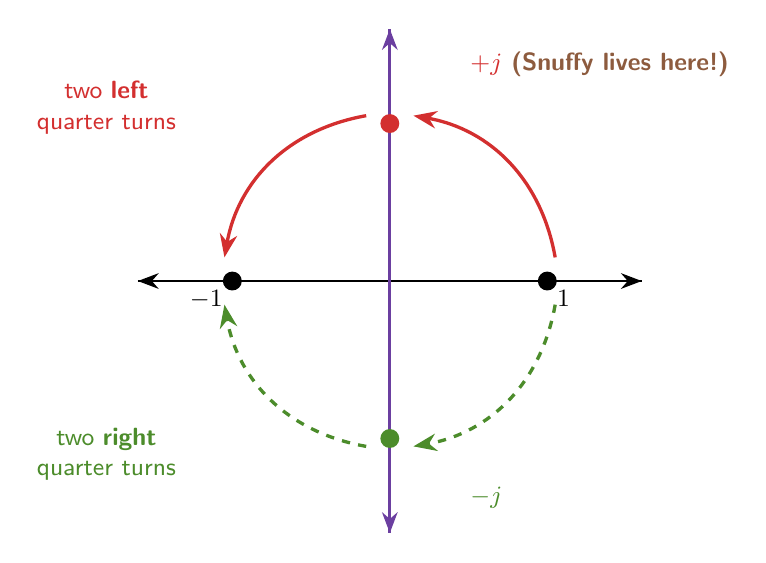
\begin{tikzpicture}[scale=1]
  \draw[-{Stealth}, line width=1pt] (-3.2,0) -- (3.2,0);
  \draw[-{Stealth}, line width=1pt] (3.2,0) -- (-3.2,0);
  \draw[-{Stealth}, line width=1pt, count] (0,-3.2) -- (0,3.2);
  \draw[-{Stealth}, line width=1pt, count] (0,3.2) -- (0,-3.2);
  \fill (2,0) circle (0.12);
  \fill (-2,0) circle (0.12);
  \fill[elmo] (0,2) circle (0.12);
  \fill[oscar] (0,-2) circle (0.12);
  \node[below right, font=\small] at (2,0) {$1$};
  \node[below left, font=\small] at (-2,0) {$-1$};
  \node[font=\small\bfseries, elmo, align=left, anchor=west] at (0.9,2.75) {$+j$ \textcolor{snuffy}{(Snuffy lives here!)}};
  \node[font=\small\bfseries, oscar, anchor=west] at (0.9,-2.75) {$-j$};
  % left turns (Elmo)
  \draw[-{Stealth}, elmo, line width=1.2pt] (2.1,0.3) to[bend right=35] (0.3,2.1);
  \draw[-{Stealth}, elmo, line width=1.2pt] (-0.3,2.1) to[bend right=35] (-2.1,0.3);
  \node[elmo, font=\small, align=center] at (-3.6,2.2) {two \textbf{left}\\quarter turns};
  % right turns (Oscar)
  \draw[-{Stealth}, oscar, line width=1.2pt, dashed] (2.1,-0.3) to[bend left=35] (0.3,-2.1);
  \draw[-{Stealth}, oscar, line width=1.2pt, dashed] (-0.3,-2.1) to[bend left=35] (-2.1,-0.3);
  \node[oscar, font=\small, align=center] at (-3.6,-2.2) {two \textbf{right}\\quarter turns};
\end{tikzpicture}
\end{center}

% ================= j = sqrt(-1) =================
\section{Meet $j$, the square root of minus one}

\begin{bigidea}
A \textbf{quarter turn to the left} is the number $\boldsymbol{j}$. It points \textbf{up}.
Two left quarter turns make a half turn, so
\[
  j \times j = -1 \qquad\text{and so}\qquad \boldsymbol{j = \sqrt{-1}}\,.
\]
Oscar's impossible tray has $j$ cookies on each side! (Engineers, who build radios and phones,
call this number $j$. Mathematicians call it $i$. Same number, different name.)
\end{bigidea}

\begin{snuffybox}
\textbf{\color{snuffy}Snuffy lives at $\boldsymbol{j}$}, one step \textbf{up}, off the number line.
For years, the grown-ups on Sesame Street said Snuffy was just Big Bird's
\textbf{imaginary} friend. But Snuffy was \textbf{real} all along!

Numbers like $j$ got the same name. A famous mathematician named Ren\'e Descartes did not
believe in them, so he called them \textbf{imaginary numbers}. But they are real and useful:
engineers use $j$ every day to build radios, phones, and power lines.
\end{snuffybox}

\question Elmo turns left twice: $j \times j = $ \blank[2cm]

\vspace{4pt}
\question Oscar turns \textbf{right} twice. That is $-j$ two times. Which way does he face at the
end? \blank[2.5cm] \quad So $(-j) \times (-j) = $ \blank[2cm]

\begin{bigidea}
So $-1$ has \textbf{two} square roots, $+j$ and $-j$, just like 9 has $+3$ and $-3$! Remember
the rule: the $\sqrt{\phantom{9}}$ sign means the \textbf{plus} one. That is why
\[
  \boldsymbol{\sqrt{-1} = +j}\,,
\]
the left turn that points \textbf{up}.
\end{bigidea}

\question Which way does $+j$ point: up or down? \blank[2cm]

\begin{mathclub}{The Count's Math Club: write it like an engineer}
Scientists and engineers write $j \times j$ as $j^2$, just like $3 \times 3 = 3^2$:
\[
  j^2 = -1, \qquad j = +\sqrt{-1}, \qquad (-j)^2 = -1 \text{ too.}
\]
\textbf{Super challenge!} $2j$ is two steps up. Check that it is the square root of $-4$:
\[
  2j \times 2j = (2 \times 2) \times (j \times j) = 4 \times (-1) = \text{\blank[1.5cm]}
\]
\end{mathclub}

\question Use the super challenge to find $\sqrt{-9}$. \quad $\sqrt{-9} = $ \blank[1.2cm]$\,j$

\begin{tcolorbox}[enhanced, colback=white, colframe=monster, boxrule=1pt, arc=3mm,
  height=4.2cm, title={\textbf{Draw it!}}, colbacktitle=monster, coltitle=white]
Draw Snuffy standing at $j$, one step up. Then draw Elmo making two left quarter turns, from
$1$ up to Snuffy and over to $-1$. Write
$j \times j = -1$ next to your picture.
\end{tcolorbox}

{\small\color{gray}\textbf{For teachers:} every nonzero number has two square roots; the
radical sign denotes the principal one, which for positive reals is the positive root and for
$-1$ is $+j$ (engineering notation; $i$ in mathematics), by convention the root at $+90^\circ$.
The turn picture is multiplication in the complex plane: $\times(-1)$ rotates by $180^\circ$ and
$\times(\pm j)$ by $\pm 90^\circ$. Caution for older students: the rule
$\sqrt{a}\sqrt{b} = \sqrt{ab}$ fails for negative $a$ and $b$, since
$\sqrt{-1}\sqrt{-1} = j^2 = -1$, not $\sqrt{1} = 1$. Next worksheet: The Cookie Circle.
Sesame Street characters appear by name only, for classroom use; this worksheet is not
affiliated with or endorsed by Sesame Workshop.}

% ================= Answer key =================
\newpage
\section{Answer key}

\begin{center}
\rowcolors{2}{white}{softyellow}
\begin{tabularx}{\linewidth}{|>{\centering\arraybackslash}p{2.8cm}|X|}
\hline
\rowcolor{cookiedark}
\textbf{\color{white}Question} & \textbf{\color{white}Answer} \\ \hline
1 & 4 sides: 16 cookies; 5 sides: 25 cookies \\ \hline
2 & $\sqrt{4} = 2$; $\sqrt{16} = 4$; $\sqrt{25} = 5$; $\sqrt{1} = 1$; $\sqrt{100} = 10$ \\ \hline
3 & 16 (a 4 by 4 tray); 12 cannot make a square \\ \hline
4 & 16 \\ \hline
5 & 5 and $-5$ \\ \hline
6 & $1$, $1$, $4$, $4$, $0$; none of them is $-1$ \\ \hline
7 & No \\ \hline
8 & $-1$ \\ \hline
9 & Backwards (toward $-1$); $(-j) \times (-j) = -1$ \\ \hline
10 & Up \\ \hline
Super challenge & $-4$, so $2j$ is a square root of $-4$ \\ \hline
11 & $3j$ (because $3j \times 3j = 9 \times (-1) = -9$) \\ \hline
\end{tabularx}
\end{center}

\end{document}
